\documentclass[a4paper]{article}

%% Page Size and Margins
\usepackage[a4paper,top=3cm,bottom=2cm,left=2cm,right=2cm,marginparwidth=1.75cm]{geometry}

%% Useful packages
\usepackage{graphicx}
\usepackage{fancyhdr}
\usepackage{hyperref}

%%\usepackage{amsmath}
%%\usepackage[colorinlistoftodos]{todonotes}
%%\usepackage[colorlinks=true, allcolors=blue]{hyperref}
%%\usepackage{caption}
%%\usepackage{subcaption}
%%\usepackage{sectsty}
%%\usepackage{apacite}
%%\usepackage{float}
%%\usepackage{titling} 
%%\usepackage{blindtext}
%%\usepackage[square,sort,comma,numbers]{natbib}
%%\usepackage[colorinlistoftodos]{todonotes}
%%\usepackage{xcolor}
%%\definecolor{darkgreen}{rgb}{0.0, 0.4, 0.0}

%% Document Begin
\begin{document}

%% titlepage
\begin{titlepage}
\vspace*{100px}
\newcommand{\HRule}{\rule{\linewidth}{0.5mm}} 	
\center 
 
% Fisrt row
{ \huge \bfseries Poor Man's Icom}
\vspace*{50px}

% Program info
\HRule \\[0.8cm]

\textsc{\normalsize \emph {A simple program that behaves like a Icom-radio}}\\[0.8cm]

\HRule \\[1cm]

%%Picture
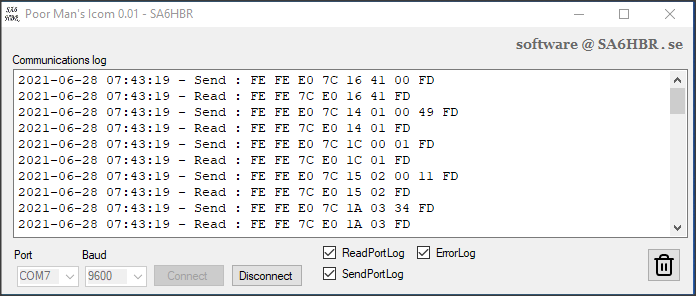
\includegraphics[width=0.6\textwidth]{../image/PoorMansIcom.png}\\[3cm] 

{\large \today}\\[2cm]
\textsc{ \huge \bfseries SA6HBR}\\[1cm]

\vfill 
\end{titlepage}

\pagestyle{fancy}
\fancyhf{}
\lhead{\today}
\rhead{SA6HBR}

%%\lhead{Guides and tutorials}
\cfoot{ \thepage}

%% Section English
%%\section*{English}

%%Simple program for displaying serial communication
%%\newpage

%% Section Svenska
\section*{Svenska}

Detta program kan man använda om man vill testa ett program som behöver en radio för att fungera.
\newline
Programmet svara som om det vore en Icom inkopplad till datorns komport. De flesta Icom använder sig av ci-v vid kommunikation, så man kan välja nästan vilken Icom som.
I samma mapp som exe-filen finns även en xml-fil som uppdateras av de meddelande som programmet skickar.
Om "Poor Man's Icom" inte svarar rätt är det i xml-filen som man får rätta till svarsmeddelandet. För att veta vad som är rätt, får man läsa "icom ci-v reference manual" för den radion man har valt. 728 använder ett fåtal meddelande. En 9100 använder många.
\vspace*{20px}
\newline
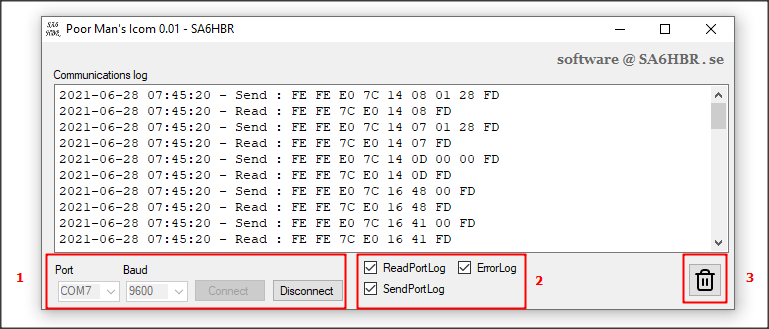
\includegraphics[width=1\textwidth]{../image/PoorMansIcomInfo.png}\\[0.5cm] 


\begin{enumerate}   
\item Inställningr för komport
\item Väljer vad som skall loggas
\item Tömmer loggrutan
\end{enumerate}  

\vspace*{50px}

\includegraphics[width=0.8\textwidth]{../image/Diagram1.png}\\[1cm] 
Normal inkoppling är att "Poor Man's Icom" kopplas via ett komportspar till programmet som skall testas.
\newline
Komportspar kan skapas med hjälp av com0com.
\newpage

\section*{XML-fil}
För att "Poor Man's Icom" skall kunna svara behöver meddelanden sparas i "IcomProtocoll.xml".
Första gång ett program skickar ett meddelande sparas det en tagg i filen. Oftast blir svaret till programmet rätt, men om det inte blir det, går det att justera.
\newline
\newline
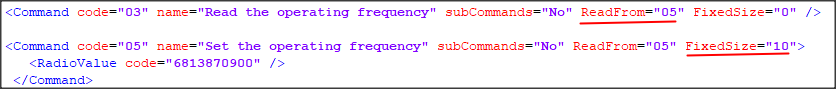
\includegraphics[width=0.8\textwidth]{../image/xml_readfrom.png}\\[0.1cm] 
När programmet frågar efter frekvensen skickar den command 03, men när programmet sätter frekvensen så skickar den på command 05.
Då sätter man ReadFrom = 05 för att command 03 skall läsa från 05. Inte alltid som programmen skickar hela frekvensen, så säkerställa att längden är rätt så sätter man FixedSize = 10.
\newline
\newline
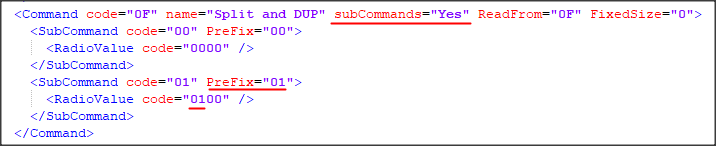
\includegraphics[width=0.8\textwidth]{../image/xml_subcommand.png}\\[0.1cm] 
Command 0F har subCommand och då sätter man subCommans=Yes.
\newline
Programmet förväntar sig svaret med subcommand + data, så då får man sätta PreFix till samma som Subcommand. Då hamnar det alltid i början på RadioValue.

\newpage

%% Section  Tested radios
\section*{Tested radios}
Tested on flrig and js8call

\begin{itemize}   
\item IC-703
\item IC-706
\item IC-718
\item IC-728
\item IC-7000
\item IC-7100
\item IC-7200
\item IC-7300
\item IC-7410
\item IC-7610
\item IC-7700
\item IC-7800
\item IC-9100
\item IC-9700
\end{itemize}  



%% Section  Useful Links
\section*{Useful Links}

* Null-modem emulator (com0com) \href{https://sourceforge.net/projects/com0com/}{https://sourceforge.net/projects/com0com/}. 

%% Section License
\section*{License}

GNU General Public License v3.0


\end{document}